\chapter{Chromatine et épigénétique}\label{ch:b3:chromatin-epigenetics}

Deux souris d'une même portée, génétiquement identiques jusqu'à la
dernière base, sont côte à côte~: l'une est mince et brune, l'autre
grasse et jaune, et elle deviendra diabétique. Une chatte tricolore
porte des plages orange et noires alors que chaque cellule de sa peau
possède les deux mêmes chromosomes~X. Un enfant hérite du même
fragment délété du chromosome~15 qu'un autre enfant, et l'un a le
syndrome de Prader--Willi tandis que l'autre a le syndrome d'Angelman
--- la seule différence tient au parent dont vient la délétion. Rien
de tout cela n'est écrit dans la séquence de l'ADN. Cela est écrit
\emph{dessus}~: dans la façon dont deux mètres d'ADN sont rangés dans
un noyau de dix micromètres, dans les petits groupements chimiques
fixés aux protéines de l'emballage et aux cytosines elles-mêmes, et
dans la machinerie qui recopie ces marques d'une cellule à ses filles.
Ce chapitre traite de cette seconde couche d'information, de ses
porteurs moléculaires et des limites honnêtes de sa mémoire.

\section{La chromatine~: l'ADN sur une bobine}

\begin{definition}[Nucléosome et chromatine]\label{def:b3:chromatin-epigenetics:nucleosome}
\index{nucléosome}\index{chromatine}\index{histone}\index{euchromatine}\index{hétérochromatine}
La \emph{chromatine} est le complexe de l'ADN et des protéines sous
lequel le génome existe dans un noyau eucaryote. Son unité répétée est
le \emph{nucléosome}~: \qty{147}{bp} d'ADN enroulés en $1.65$ tour
lévogyre autour d'un octamère d'\emph{histones} --- deux exemplaires
de chacune des petites protéines très basiques H2A, H2B, H3 et H4 ---
suivis d'un \emph{ADN de liaison} de \qtyrange{20}{60}{bp} jusqu'au
nucléosome suivant. Une cinquième histone, H1, se fixe sur cet ADN de
liaison là où il entre dans le cœur et en sort, et aide les perles à
s'empiler les unes contre les autres. Chaque histone du cœur porte une
\emph{queue} amino-terminale non structurée d'une \numrange{20}{40}
résidus, qui fait saillie hors de la particule. La chromatine qui se
colore faiblement, reste peu compactée et est transcrite est
l'\emph{euchromatine}~; celle qui est dense, de réplication tardive et
largement silencieuse --- aux centromères, aux télomères et sur les
séquences répétées --- est l'\emph{hétérochromatine}.
\end{definition}

\begin{proof}[Faits expérimentaux]
Hewish et Burgoyne (1973) ont digéré des noyaux de foie de rat par une
nucléase endogène et ont trouvé que l'ADN en sortait non pas comme une
traînée continue, mais comme une échelle de fragments dont les
longueurs étaient des multiples d'environ \qty{200}{bp}~: l'ADN était
protégé à intervalles réguliers et coupé seulement entre eux. Kornberg
(1974) a montré que l'unité protégée était une particule de huit
\omterm{def:b3:chromatin-epigenetics:nucleosome}{histones} portant environ \qty{200}{bp}, et les micrographies
électroniques de \omterm{def:b3:chromatin-epigenetics:nucleosome}{chromatine} délicatement étalée montraient le
«~collier de perles~». Luger et ses collègues (1997) ont résolu la
structure cristalline de la particule cœur à \qty{2.8}{\angstrom}~:
\qty{147}{bp}, un octamère dont les queues passent entre les tours
d'ADN.
\end{proof}

\begin{omfigure}
\begin{tikzpicture}[every node/.style={font=\scriptsize}, >=stealth]
  % beads on a string
  \foreach \x/\y in {0/0, 2.2/0.5, 4.4/0, 6.6/0.5, 8.8/0} {
    \fill[omDef!30] (\x,\y) circle (0.42);
    \draw[very thick, omThm!70!black] (\x,\y) circle (0.5);
  }
  \draw[very thick, omThm!70!black] (-1.1,-0.1) -- (0-0.47,-0.17);
  \draw[very thick, omThm!70!black] (0.47,-0.17) -- (2.2-0.47,0.33);
  \draw[very thick, omThm!70!black] (2.67,0.33) -- (4.4-0.47,-0.17);
  \draw[very thick, omThm!70!black] (4.87,-0.17) -- (6.6-0.47,0.33);
  \draw[very thick, omThm!70!black] (7.07,0.33) -- (8.8-0.47,-0.17);
  \draw[very thick, omThm!70!black] (9.27,-0.17) -- (10.4,-0.1);
  % tails
  \foreach \x/\y in {0/0, 4.4/0, 8.8/0} { \draw[omProp, thick] (\x,\y+0.5) .. controls (\x-0.2,\y+0.9) .. (\x+0.1,\y+1.15); \draw[omProp, thick] (\x,\y-0.5) .. controls (\x+0.2,\y-0.9) .. (\x-0.1,\y-1.15); }
  \foreach \x/\y in {2.2/0.5, 6.6/0.5} { \draw[omProp, thick] (\x,\y+0.5) .. controls (\x-0.2,\y+0.9) .. (\x+0.1,\y+1.15); }
  % H1
  \fill[omMeth!70!black] (1.55,0.05) circle (0.12); \fill[omMeth!70!black] (5.95,0.05) circle (0.12);
  % labels
  \node[above, align=center] at (2.2,1.75) {queues d'histones\\(acétylation, méthylation)};
  \node[below, align=center] at (4.4,-1.35) {particule cœur~: octamère\\$+$ \qty{147}{bp}, $1.65$ tour};
  \node[below, align=center] at (7.7,-0.55) {ADN de liaison\\\qtyrange{20}{60}{bp}};
  \node[below] at (5.95,-0.1) {H1};
  \draw[<->] (-0.5,-2.2) -- (2.2-0.5,-2.2) node[midway, below] {répétition $\approx \qty{200}{bp}$, \qty{11}{nm}};
  \draw[gray] (-0.5,-1.95) -- (-0.5,-2.35); \draw[gray] (1.7,-1.95) -- (1.7,-2.35);
\end{tikzpicture}

{\small La fibre de \qty{10}{nm}~: des cœurs de \omterm{def:b3:chromatin-epigenetics:nucleosome}{nucléosomes} (bleu) sur
un ADN continu (rouge), chaque perle étant un octamère d'\omterm{def:b3:chromatin-epigenetics:nucleosome}{histones} dont
les queues (orange) font saillie, avec l'\omterm{def:b3:chromatin-epigenetics:nucleosome}{histone} de liaison H1 (vert)
au point d'entrée et de sortie. Six \omterm{def:b3:chromatin-epigenetics:nucleosome}{nucléosomes} environ occupent la
longueur que prendraient \qty{1200}{bp} d'ADN nu.}
\end{omfigure}

\begin{omfigure}
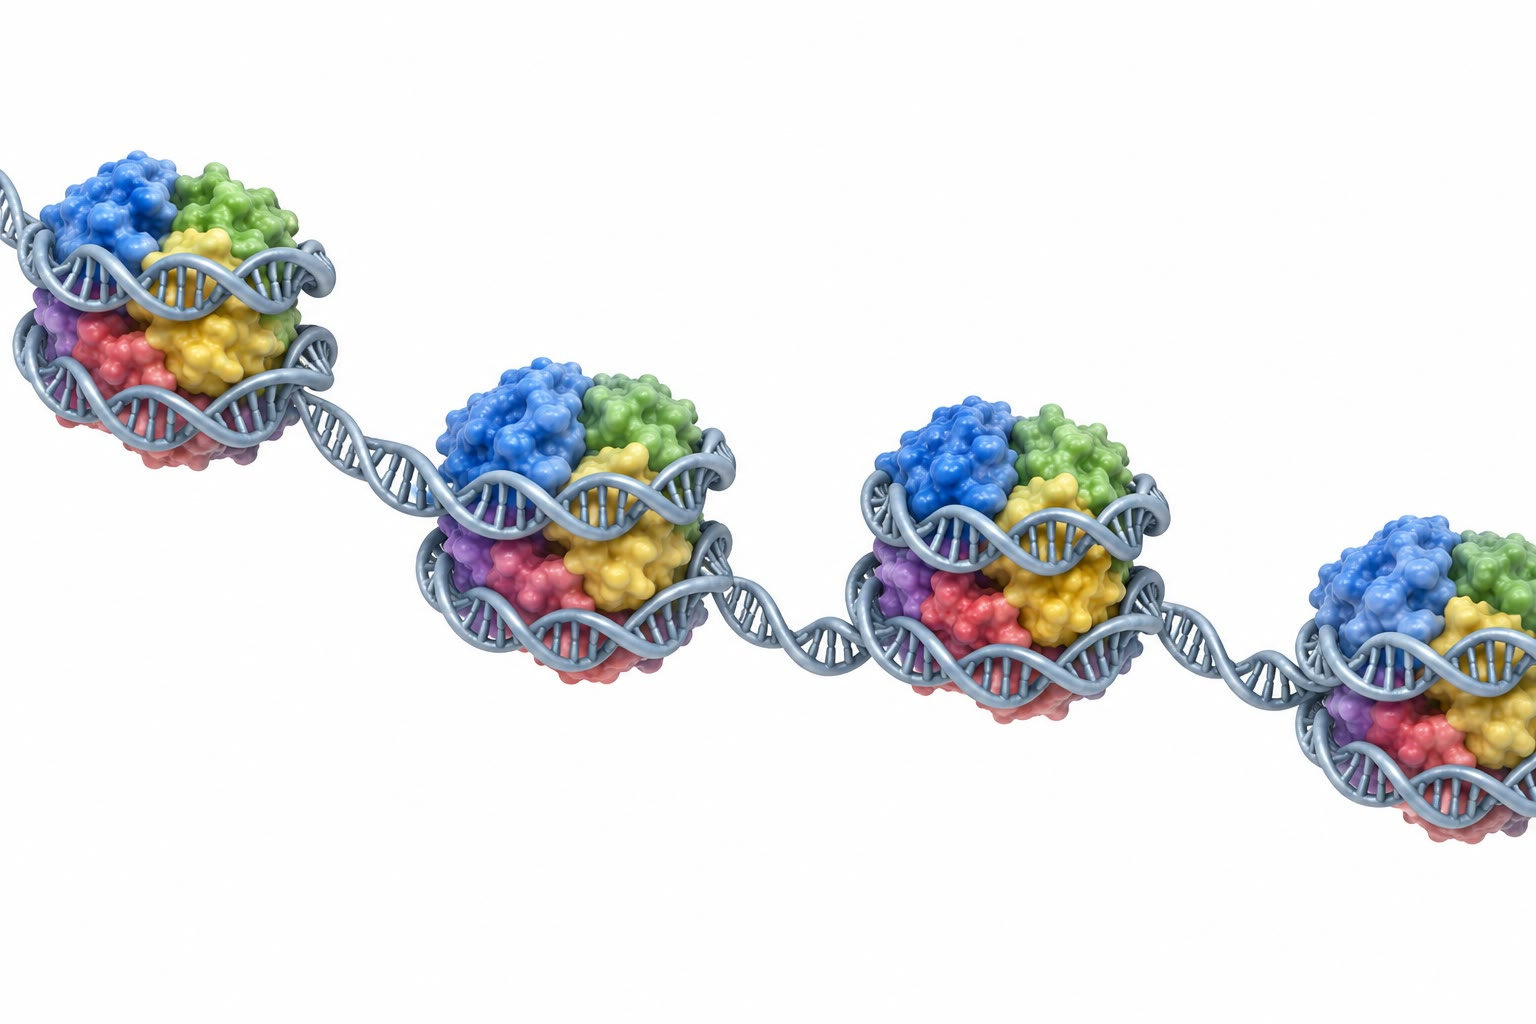
\includegraphics[width=0.6\linewidth]{images/book5/ai/b5-01-nucleosomes.jpg}

{\small La \omterm{def:b3:chromatin-epigenetics:nucleosome}{chromatine} à l'échelle moléculaire~: la double hélice
enroulée autour de cœurs d'\omterm{def:b3:chromatin-epigenetics:nucleosome}{histones} successifs, le «~collier de
perles~» que révélait l'échelle de fragments de la nucléase.}
\end{omfigure}

\begin{proposition}[Niveaux de compaction]\label{prop:b3:chromatin-epigenetics:compaction}
\index{taux de compaction}\index{boucle de chromatine}\index{domaine d'association topologique}
Le \emph{\omterm{prop:b3:chromatin-epigenetics:compaction}{taux de compaction}} d'une structure de \omterm{def:b3:chromatin-epigenetics:nucleosome}{chromatine} est la
longueur de l'ADN qu'elle contient divisée par la longueur de la
structure. L'enroulement en fibre de \qty{10}{nm} donne un rapport
voisin de $6$~: les \qty{68}{nm} d'une répétition de \qty{200}{bp}
sont comprimés en une perle de \qty{11}{nm}. Dans le noyau
interphasique la fibre n'est pas enroulée en une fibre régulière plus
épaisse, comme les manuels l'ont longtemps dessinée, mais repliée en
\emph{boucles} de dizaines à centaines de kilobases, tenues à leur
base par les complexes annulaires de cohésine et par la protéine CTCF,
qui se lie à l'ADN~; les boucles se regroupent en \emph{\omterm{prop:b3:chromatin-epigenetics:compaction}{domaines
d'association topologique}} (TAD) d'environ une mégabase, au sein
desquels un gène rencontre ses régulateurs bien plus souvent qu'il ne
rencontre quoi que ce soit au dehors. Un chromosome mitotique, l'état
le plus compact, a un \omterm{prop:b3:chromatin-epigenetics:compaction}{taux de compaction} voisin de \num{10000}~: les
\qty{4}{cm} d'ADN d'un chromosome humain moyen sont repliés en un
bâtonnet long de \qty{4}{\micro m}.
\end{proposition}

\begin{example}[Deux mètres dans dix micromètres]\label{ex:b3:chromatin-epigenetics:two-metres}
Un noyau diploïde humain contient $6.4\times 10^{9}$ paires de bases. À
\qty{0.34}{nm} par paire de bases cela fait \qty{2.2}{m} de double
hélice, dans un noyau d'environ \qty{10}{\micro m} de diamètre. Cet ADN
est rangé en $6.4\times 10^{9}/200 \approx 3.2\times 10^{7}$
\omterm{def:b3:chromatin-epigenetics:nucleosome}{nucléosomes}, portant chacun environ \qty{108}{kDa} d'\omterm{def:b3:chromatin-epigenetics:nucleosome}{histones} contre
\qty{96}{kDa} d'ADN (\qty{147}{bp} à \qty{650}{Da} la paire)~: le noyau
contient à peu près autant d'\omterm{def:b3:chromatin-epigenetics:nucleosome}{histones} que d'ADN en masse. L'ADN
lui-même, traité comme un cylindre de \qty{2}{nm} de diamètre, n'occupe
qu'environ \qty{7}{\micro m^3}, soit quelque \qty{1}{\%} d'un noyau
sphérique de rayon \qty{5}{\micro m}~; le problème de l'emballage est
un problème d'enchevêtrement et d'accès, non de place.
\end{example}

\section{Le code des histones}

\begin{definition}[Modifications des histones]\label{def:b3:chromatin-epigenetics:histone-code}
\index{code des histones}\index{acétylation}\index{méthylation des histones}\index{écrivain}\index{lecteur}\index{effaceur}
Les résidus des queues d'\omterm{def:b3:chromatin-epigenetics:nucleosome}{histones} sont modifiés de façon covalente~:
\emph{acétylation} des lysines (qui neutralise leur charge positive et
relâche la prise sur l'ADN), \emph{méthylation} des lysines et des
arginines (un, deux ou trois groupements méthyle, sans changement de
charge), phosphorylation des sérines, ubiquitinylation des lysines. Une
modification se nomme par l'\omterm{def:b3:chromatin-epigenetics:nucleosome}{histone}, le résidu et le groupement~:
H3K4me3 désigne l'\omterm{def:b3:chromatin-epigenetics:nucleosome}{histone} H3, lysine~4, triméthylée~; H3K27ac, H3 dont
la lysine~27 est acétylée. Le \emph{code des \omterm{def:b3:chromatin-epigenetics:nucleosome}{histones}} est la
corrélation entre des combinaisons de marques et l'état du gène
sous-jacent~: H3K4me3 et H3K27ac sur les promoteurs et les amplificateurs
actifs, H3K36me3 le long du corps des gènes transcrits, H3K9me3 sur
l'\omterm{def:b3:chromatin-epigenetics:nucleosome}{hétérochromatine} constitutive, H3K27me3 sur les gènes réprimés au
cours du développement. Les enzymes qui déposent une marque sont des
\emph{écrivains} (histone-acétyltransférases, HAT~; méthyltransférases),
celles qui la retirent des \emph{effaceurs} (histone-désacétylases,
HDAC~; déméthylases), et les protéines qui reconnaissent une marque et
agissent sur elle des \emph{lecteurs}~: un \emph{bromodomaine} lie une
acétyl-lysine, un \emph{chromodomaine} une méthyl-lysine.
\end{definition}

\begin{proposition}[Les marques sont lues, non pas seulement subies]\label{prop:b3:chromatin-epigenetics:readers}
\index{HP1}\index{Polycomb}\index{PRC2}\index{Trithorax}
L'\omterm{def:b3:chromatin-epigenetics:histone-code}{acétylation} agit en partie par électrostatique --- une queue acétylée
retient moins fortement son ADN et la fibre s'ouvre --- mais la plupart
des marques agissent en recrutant des \omterm{def:b3:chromatin-epigenetics:histone-code}{lecteurs}. H3K9me3 est liée par le
chromodomaine de la \emph{protéine de l'\omterm{def:b3:chromatin-epigenetics:nucleosome}{hétérochromatine} HP1}, qui se
dimérise, ponte des \omterm{def:b3:chromatin-epigenetics:nucleosome}{nucléosomes} voisins et recrute la
méthyltransférase (SUV39H) qui écrit H3K9me3 sur le \omterm{def:b3:chromatin-epigenetics:nucleosome}{nucléosome}
suivant~: la marque se propage le long de la fibre jusqu'à rencontrer
une frontière, et compacte ce qu'elle couvre. H3K27me3 est écrite par
le \emph{complexe répresseur Polycomb 2} (PRC2, sous-unité catalytique
EZH2) et lue par PRC1, qui ubiquitinyle H2A et compacte la fibre~; le
complexe est lui-même stimulé par la marque qu'il dépose. Le groupe
\emph{Trithorax} écrit la marque opposée H3K4me3 et maintient actifs
les gènes du développement propres à un type cellulaire donné. Chacune
de ces boucles --- un \omterm{def:b3:chromatin-epigenetics:histone-code}{lecteur} qui recrute un \omterm{def:b3:chromatin-epigenetics:histone-code}{écrivain} --- est une
rétroaction positive qui permet à un état de se maintenir une fois
établi, ce dont une marque héritable a besoin.
\end{proposition}

\begin{omfigure}
\begin{tikzpicture}[every node/.style={font=\scriptsize}, >=stealth]
  % nucleosomes with tails
  \foreach \x in {0,2,4,6} { \draw[thick, omDef, fill=omDef!20] (\x,0) circle (0.45); \draw[omProp, thick] (\x,0.45) -- (\x,1.15); }
  % marks
  \fill[omThm] (2,1.15) circle (0.11); \fill[omThm] (4,1.15) circle (0.11);
  \fill[omMeth!80!black] (0,1.15) circle (0.11);
  \node[left] at (-0.5,1.15) {ac};
  \node[right, align=left] at (6.15,1.15) {me3};
  % HP1 reader
  \draw[thick, fill=omExo!30] (2.6,1.7) ellipse (0.5 and 0.25); \node at (2.6,1.7) {lecteur};
  \draw[thick, fill=omExo!30] (4.2,2.35) ellipse (0.55 and 0.25); \node at (4.2,2.35) {écrivain};
  \draw[->, thick] (2.9,1.9) -- (3.75,2.2);
  \draw[->, thick, omThm] (4.6,2.15) .. controls (5.6,2.0) and (6.1,1.8) .. (6.05,1.3);
  \node[right, align=left, font=\scriptsize] at (6.6,2.0) {se propage au\\nucléosome suivant};
  \draw[->, thick, gray] (2.2,1.3) -- (2.45,1.5);
  % eraser
  \draw[thick, fill=omExo!30] (0.6,2.2) ellipse (0.5 and 0.25); \node at (0.6,2.2) {effaceur};
  \draw[->, thick, omMeth!80!black] (0.3,2.0) -- (0.05,1.35);
  % DNA
  \draw[very thick, omThm!70!black] (-0.9,-0.3) -- (-0.45,-0.05) (0.45,-0.05) -- (1.55,-0.05) (2.45,-0.05) -- (3.55,-0.05) (4.45,-0.05) -- (5.55,-0.05) (6.45,-0.05) -- (7.2,-0.3);
  \node[below, align=center] at (0,-0.6) {ouvert~: l'acétyle\\supprime une charge};
  \node[below, align=center] at (5,-0.6) {fermé~: H3K9me3 lue par HP1,\\qui recrute la méthylase K9};
\end{tikzpicture}

{\small La logique écrivain--lecteur--effaceur. Un \omterm{def:b3:chromatin-epigenetics:histone-code}{lecteur} fixé sur une
marque portée par un \omterm{def:b3:chromatin-epigenetics:nucleosome}{nucléosome} recrute l'\omterm{def:b3:chromatin-epigenetics:histone-code}{écrivain} qui dépose la même
marque sur le suivant, de sorte que l'état se propage et se recopie~;
les \omterm{def:b3:chromatin-epigenetics:histone-code}{effaceurs} s'y opposent. Les groupements acétyle (vert) ouvrent la
fibre, H3K9me3 (rouge) la ferme.}
\end{omfigure}

\begin{method}[Immunoprécipitation de la chromatine (ChIP)]\label{met:b3:chromatin-epigenetics:chip}
\index{ChIP}\index{immunoprécipitation de la chromatine}
Pour cartographier l'emplacement d'une marque ou d'une protéine sur le
génome~: (1) pontage des protéines à l'ADN dans des cellules vivantes
par le formaldéhyde~; (2) fragmentation de la \omterm{def:b3:chromatin-epigenetics:nucleosome}{chromatine} en morceaux de
quelques centaines de paires de bases~; (3) précipitation des fragments
par un anticorps dirigé contre la marque (par exemple H3K27me3) et fixé
sur des billes~; (4) rupture des pontages et purification de l'ADN~;
(5) séquençage (ChIP-seq) et comptage des lectures le long du génome~:
les pics sont les endroits où se trouvait la marque. Un témoin d'ADN
d'entrée, sans anticorps, fixe le bruit de fond. La résolution est
celle des fragments, environ un \omterm{def:b3:chromatin-epigenetics:nucleosome}{nucléosome}.
\end{method}

\begin{remark}[Code ou corrélation]\label{rem:b3:chromatin-epigenetics:code}
Le mot «~code~» va trop loin. Beaucoup de marques sont des conséquences
de la transcription plutôt que ses causes (H3K36me3 est déposée par une
méthyltransférase qui voyage avec la polymérase), et supprimer un
\omterm{def:b3:chromatin-epigenetics:histone-code}{écrivain} change souvent l'expression bien moins que la distribution de
la marque ne le laisse croire. Ce qui est bien établi, c'est que
quelques marques --- H3K9me3, H3K27me3 et la \omterm{def:b3:chromatin-epigenetics:methylation}{méthylation de l'ADN}
ci-dessous --- portent une répression qui s'auto-entretient et survit
au signal qui l'a installée.
\end{remark}

\section{Méthylation de l'ADN et recopie d'une marque}

\begin{definition}[Méthylation de l'ADN]\label{def:b3:chromatin-epigenetics:methylation}
\index{méthylation de l'ADN}\index{CpG}\index{îlot CpG}\index{DNMT1}\index{méthylation de maintenance}\index{méthylation de novo}
Chez les vertébrés, un groupement méthyle est ajouté sur le carbone~5
d'une cytosine presque uniquement dans le dinucléotide \emph{CpG} (un C
suivi d'un G sur le même brin), séquence qui est son propre
complémentaire, de sorte qu'un CpG méthylé l'est normalement sur les
deux brins. De \qtyrange{70}{80}{\%} des CpG d'une cellule humaine sont
méthylés, et les promoteurs méthylés sont silencieux~: les groupements
méthyle sont lus par des protéines à domaine de liaison au méthyl-CpG
(MeCP2, MBD1--4) qui recrutent des HDAC et des méthylases de H3K9, et
ils bloquent directement plusieurs facteurs de transcription. Font
exception les \emph{îlots CpG}, régions d'environ une kilobase, riches
en G et en C et en CpG, qui occupent le promoteur de la plupart des
gènes de ménage et restent non méthylées dans une cellule normale. Le
groupement méthyle est déposé par les \emph{ADN-méthyltransférases}~:
DNMT3A et DNMT3B assurent la \emph{méthylation de novo} des sites non
méthylés, et \emph{DNMT1}, qui préfère un CpG hémiméthylé --- un brin
méthylé, l'autre non --- assure la \emph{méthylation de maintenance}
derrière la fourche de réplication. Le retrait est passif, par
réplication sans maintenance, ou actif, par les enzymes TET, qui
oxydent la 5-méthylcytosine en 5-hydroxyméthylcytosine et au-delà,
jusqu'à ce que la réparation par excision de base la remplace par une
cytosine ordinaire.
\end{definition}

\begin{example}[Pourquoi le génome est pauvre en CpG]\label{ex:b3:chromatin-epigenetics:cpg-deficit}
Le génome humain contient \qty{42}{\%} de G$+$C~; si les bases étaient
indépendantes, un \omterm{def:b3:chromatin-epigenetics:methylation}{CpG} surviendrait à la fréquence
$0.21\times 0.21 \approx 0.044$, soit environ $2.8\times 10^{8}$ fois
dans le génome diploïde. Le nombre observé est d'environ
$5.6\times 10^{7}$, un cinquième de cela. La raison en est la marque
elle-même~: une cytosine méthylée qui perd son groupement aminé devient
une thymine, base normale que la réparation ne peut reconnaître comme
fautive, alors qu'une cytosine non méthylée se désamine en uracile, qui
est excisé. Au fil du temps évolutif les \omterm{def:b3:chromatin-epigenetics:methylation}{CpG} méthylés ont muté en TpG
et CpA, et seuls les îlots non méthylés ont gardé leurs \omterm{def:b3:chromatin-epigenetics:methylation}{CpG}. La marque
a laissé sa signature dans la séquence.
\end{example}

\begin{theorem}[Maintien d'un état de méthylation au fil des divisions]\label{thm:b3:chromatin-epigenetics:maintenance}
\index{mémoire épigénétique}\index{chaîne de Markov!méthylation}
Considérons un site \omterm{def:b3:chromatin-epigenetics:methylation}{CpG}, suivi le long d'une lignée de cellules. À
chaque division, la cytosine du brin néoformé est méthylée avec la
probabilité $\mu$ si celle du brin matrice l'est (efficacité de
maintenance) et avec la probabilité $\delta$ si elle ne l'est pas (taux
de novo). Soit $p_{n}$ la probabilité que le site soit méthylé après
$n$ divisions. Alors
\[
p_{n+1} = \mu\, p_{n} + \delta\,(1 - p_{n}),
\qquad
p_{n} = p^{*} + (p_{0} - p^{*})\,(\mu - \delta)^{n},
\qquad
p^{*} = \frac{\delta}{1 - \mu + \delta}.
\]
Tout site dérive vers le même équilibre $p^{*}$, quel que soit son état
de départ, et la mémoire de l'état initial décroît géométriquement de
raison $\mu - \delta$. Une marque est retenue pendant environ
$1/(1 - \mu + \delta)$ divisions~; la mémoire fidèle d'une
\emph{différence} entre sites exige donc $\mu$ très proche de $1$ et
$\delta$ très proche de $0$, ou bien une rétroaction qui fasse dépendre
$\mu$ et $\delta$ de l'état du voisinage.
\end{theorem}
\begin{proof}
La récurrence est la formule des probabilités totales sur les deux
états du brin matrice. Son point fixe vérifie $p^{*} = \mu p^{*} + \delta(1 -
p^{*})$, d'où $p^{*}(1 - \mu + \delta) = \delta$. En retranchant
l'équation du point fixe de la récurrence, $p_{n+1} - p^{*} = (\mu -
\delta)(p_{n} - p^{*})$, qui s'itère en la forme close. Comme
$0 \le \delta \le \mu \le 1$, la raison $\mu - \delta$ appartient à $[0,1]$
et l'écart décroît~; il est divisé par deux toutes les $\ln 2 / (-\ln(\mu -
\delta)) \approx \ln 2/(1 - \mu + \delta)$ divisions lorsque $\mu -
\delta$ est proche de $1$.
\end{proof}

\begin{example}[Les nombres]\label{ex:b3:chromatin-epigenetics:maintenance-numbers}
Les valeurs mesurées sur des cellules de mammifère sont
$\mu \approx 0.99$ et $\delta \approx 0.02$ par division sur un \omterm{def:b3:chromatin-epigenetics:methylation}{CpG}
ordinaire. On a alors $p^{*} =
0.02/0.03 \approx 0.67$, proche de la fraction méthylée à l'échelle du
génome entier, et $\mu - \delta = 0.97$~: un site entièrement méthylé,
laissé à la seule machinerie, serait revenu à mi-chemin de la moyenne
après $\ln 2 /
0.03 \approx 23$ divisions. Un promoteur réprimé qui doit le rester
pendant les centaines de divisions d'une vie a donc besoin de plus que
\omterm{def:b3:chromatin-epigenetics:methylation}{DNMT1}~: les \omterm{def:b3:chromatin-epigenetics:histone-code}{lecteurs} du \omterm{def:b3:chromatin-epigenetics:methylation}{méthyl-CpG} recrutent la méthylation de H3K9 et
les \omterm{def:b3:chromatin-epigenetics:histone-code}{lecteurs} de H3K9 recrutent DNMT3, si bien qu'un îlot dense de
marques élève son propre $\mu$ vers $1$ et abaisse le $\delta$ du
voisinage vers $0$. À l'inverse, une cellule qui perd \omterm{def:b3:chromatin-epigenetics:methylation}{DNMT1} perd la
marque passivement~: avec $\mu = \delta = 0$ la fraction de brins
méthylés est divisée par deux à chaque division.
\end{example}

\begin{omfigure}
\begin{tikzpicture}[every node/.style={font=\scriptsize}, >=stealth]
  % left: replication scheme
  \begin{scope}
    \draw[very thick, omThm!70!black] (0,1.2) -- (2.4,1.2); \draw[very thick, omThm!70!black] (0,0.9) -- (2.4,0.9);
    \foreach \x in {0.5,1.2,1.9} { \fill[omDef] (\x,1.2) circle (0.09); \fill[omDef] (\x,0.9) circle (0.09); }
    \node[above] at (1.2,1.3) {parental~: les deux brins méthylés};
    \draw[->, thick] (1.2,0.75) -- (1.2,0.15) node[midway, right] {réplication};
    \draw[very thick, omThm!70!black] (0,-0.1) -- (2.4,-0.1); \draw[very thick, gray] (0,-0.4) -- (2.4,-0.4);
    \foreach \x in {0.5,1.2,1.9} { \fill[omDef] (\x,-0.1) circle (0.09); \draw[omDef] (\x,-0.4) circle (0.09); }
    \node[left] at (-0.1,-0.25) {hémiméthylé};
    \draw[->, thick] (1.2,-0.85) -- (1.2,-1.45) node[midway, right, align=left] {DNMT1, probabilité $\mu$\\par site};
    \draw[very thick, omThm!70!black] (0,-1.7) -- (2.4,-1.7); \draw[very thick, gray] (0,-2.0) -- (2.4,-2.0);
    \foreach \x in {0.5,1.9} { \fill[omDef] (\x,-1.7) circle (0.09); \fill[omDef] (\x,-2.0) circle (0.09); }
    \fill[omDef] (1.2,-1.7) circle (0.09); \draw[omDef] (1.2,-2.0) circle (0.09);
    \node[below, align=center] at (1.2,-2.1) {rétabli, un site manqué~:\\le brin neuf de la fille};
  \end{scope}
  % right: decay plot
  \begin{scope}[xshift=5.0cm, yshift=-2.3cm]
  \begin{axis}[
    width=6.6cm, height=4.6cm, axis lines=left,
    xmin=0, xmax=100, ymin=0, ymax=1.05,
    xlabel={divisions $n$},
    xlabel style={font=\scriptsize, at={(axis description cs:0.5,-0.1)}, anchor=north},
    tick label style={font=\scriptsize}, xtick={0,25,50,75,100}, ytick={0,0.5,0.67,1},
    yticklabels={0,0.5,$p^{*}$,1}, clip=false,
  ]
  \addplot[very thick, omDef, domain=0:100, samples=60] {0.6667 + 0.3333*0.97^x};
  \addplot[very thick, omThm, domain=0:100, samples=60] {0.6667 - 0.6667*0.97^x};
  \addplot[dashed, gray, domain=0:100, samples=2] {0.6667};
  \addplot[thick, omMeth!80!black, domain=0:100, samples=60] {0.6667 + 0.3333*0.998^x};
  \node[font=\scriptsize] at (axis cs:-9,1.1) {$p_{n}$};
  \node[font=\scriptsize, omDef, anchor=south west] at (axis cs:45,0.82) {départ méthylé, $\mu = 0.99$};
  \node[font=\scriptsize, omThm, anchor=north west] at (axis cs:50,0.30) {départ non méthylé};
  \node[font=\scriptsize, omMeth!80!black, anchor=south west] at (axis cs:30,1.02) {avec rétroaction, $\mu = 0.999$};
  \end{axis}
  \end{scope}
\end{tikzpicture}

{\small À gauche~: la \omterm{def:b3:chromatin-epigenetics:methylation}{méthylation de maintenance}. Après réplication
chaque \omterm{def:b3:chromatin-epigenetics:methylation}{CpG} est hémiméthylé~; \omterm{def:b3:chromatin-epigenetics:methylation}{DNMT1} recopie la marque sur le brin neuf
avec la probabilité $\mu$ par site. À droite~: le devenir d'un site au
fil des divisions pour $\mu = 0.99$, $\delta = 0.02$ (bleu depuis
l'état méthylé, rouge depuis l'état non méthylé) --- tous deux
convergent vers $p^{*} = 0.67$ --- et pour un site dont la rétroaction
de voisinage porte $\mu$ à $0.999$ (vert).}
\end{omfigure}

\begin{method}[Lire la méthylation~: le séquençage après bisulfite]\label{met:b3:chromatin-epigenetics:bisulfite}
\index{séquençage après bisulfite}
Le séquençage seul ne voit pas un groupement méthyle. On traite l'ADN
dénaturé par le bisulfite de sodium~: une cytosine non méthylée est
désaminée en uracile, qui se lit T après PCR, tandis qu'une
5-méthylcytosine est protégée et se lit toujours C. On séquence l'ADN
converti et on le compare à la référence~: tout C resté C était
méthylé, tout C devenu T ne l'était pas. Appliqué à l'ensemble du
génome (\omterm{met:b3:chromatin-epigenetics:bisulfite}{séquençage après bisulfite} du génome entier), le procédé donne
l'état de méthylation de chacun des $2.8\times 10^{7}$ \omterm{def:b3:chromatin-epigenetics:methylation}{CpG} d'un génome
haploïde à la base près, sous forme d'une fraction des cellules de
l'échantillon.
\end{method}

\section{Inactivation de l'X et empreinte parentale}

\begin{definition}[Inactivation du chromosome~X]\label{def:b3:chromatin-epigenetics:x-inactivation}
\index{inactivation de l'X}\index{corpuscule de Barr}\index{Xist}\index{compensation de dose}
Chez les mammifères femelles, l'un des deux chromosomes~X de chaque
cellule somatique est réduit au silence transcriptionnel tôt dans le
développement, forme de \emph{compensation de dose} qui égalise
l'expression des gènes liés à l'X entre les femelles~XX et les
mâles~XY. Le chromosome réprimé est compacté en un corps dense contre
l'enveloppe nucléaire, le \emph{corpuscule de Barr}. Le choix de l'X à
réprimer est aléatoire dans l'embryon proprement dit et, une fois fait,
il est transmis clonalement à toute la descendance de la cellule.
L'inactivation est déclenchée par \emph{Xist}, un ARN non codant de
\qty{17}{kb} transcrit depuis le centre d'inactivation du chromosome
qui sera réprimé~: il recouvre ce chromosome en cis, recrute Polycomb
(H3K27me3), le variant d'\omterm{def:b3:chromatin-epigenetics:nucleosome}{histone} macroH2A puis la \omterm{def:b3:chromatin-epigenetics:methylation}{méthylation de l'ADN}
des promoteurs, et le silence se maintient ensuite sans que Xist soit
nécessaire à chaque division. Environ \qty{15}{\%} des gènes humains
liés à l'X échappent à l'inactivation, en partie ou en totalité.
\end{definition}

\begin{proof}[Faits expérimentaux]
Barr et Bertram (1949) ont remarqué un corps dense dans le noyau des
neurones de chatte, absent chez le chat. Ohno (1959) a montré que
c'était un chromosome~X entier, condensé. Lyon (1961) a rassemblé les
pièces~: les souris femelles hétérozygotes pour des gènes de couleur du
pelage liés à l'X ont un pelage en mosaïque, fait de plages exprimant
l'un ou l'autre allèle, donc chaque plage est un clone où le même X est
silencieux~; il en va de même des plages orange et noires d'une chatte
écaille de tortue ou tricolore, dont le gène orange est lié à l'X, et
des glandes sudoripares en mosaïque des femmes porteuses d'un allèle
muté d'un gène lié à l'X. Un chat tricolore mâle est presque toujours
XXY.
\end{proof}

\begin{omfigure}
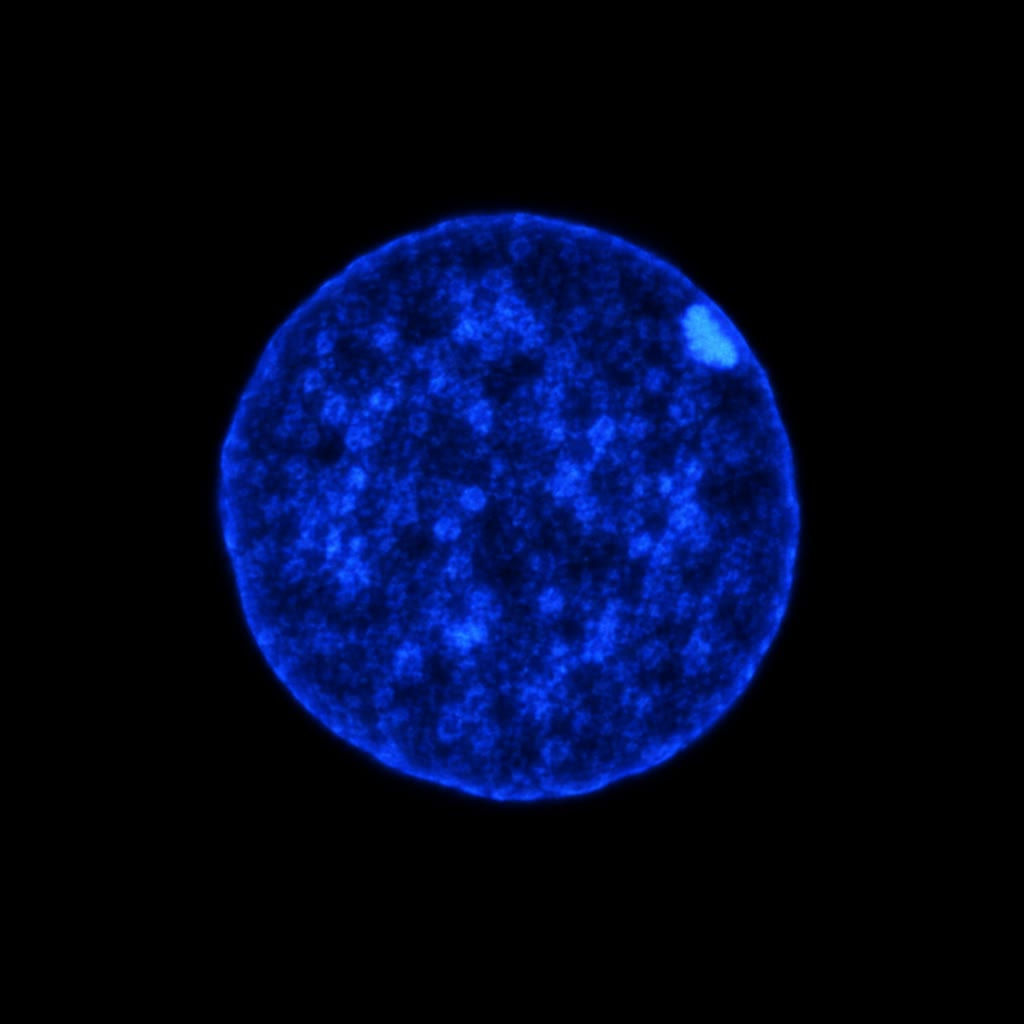
\includegraphics[width=0.42\linewidth]{images/book5/ai/b5-01-barr-body.jpg}\hspace{0.04\linewidth}
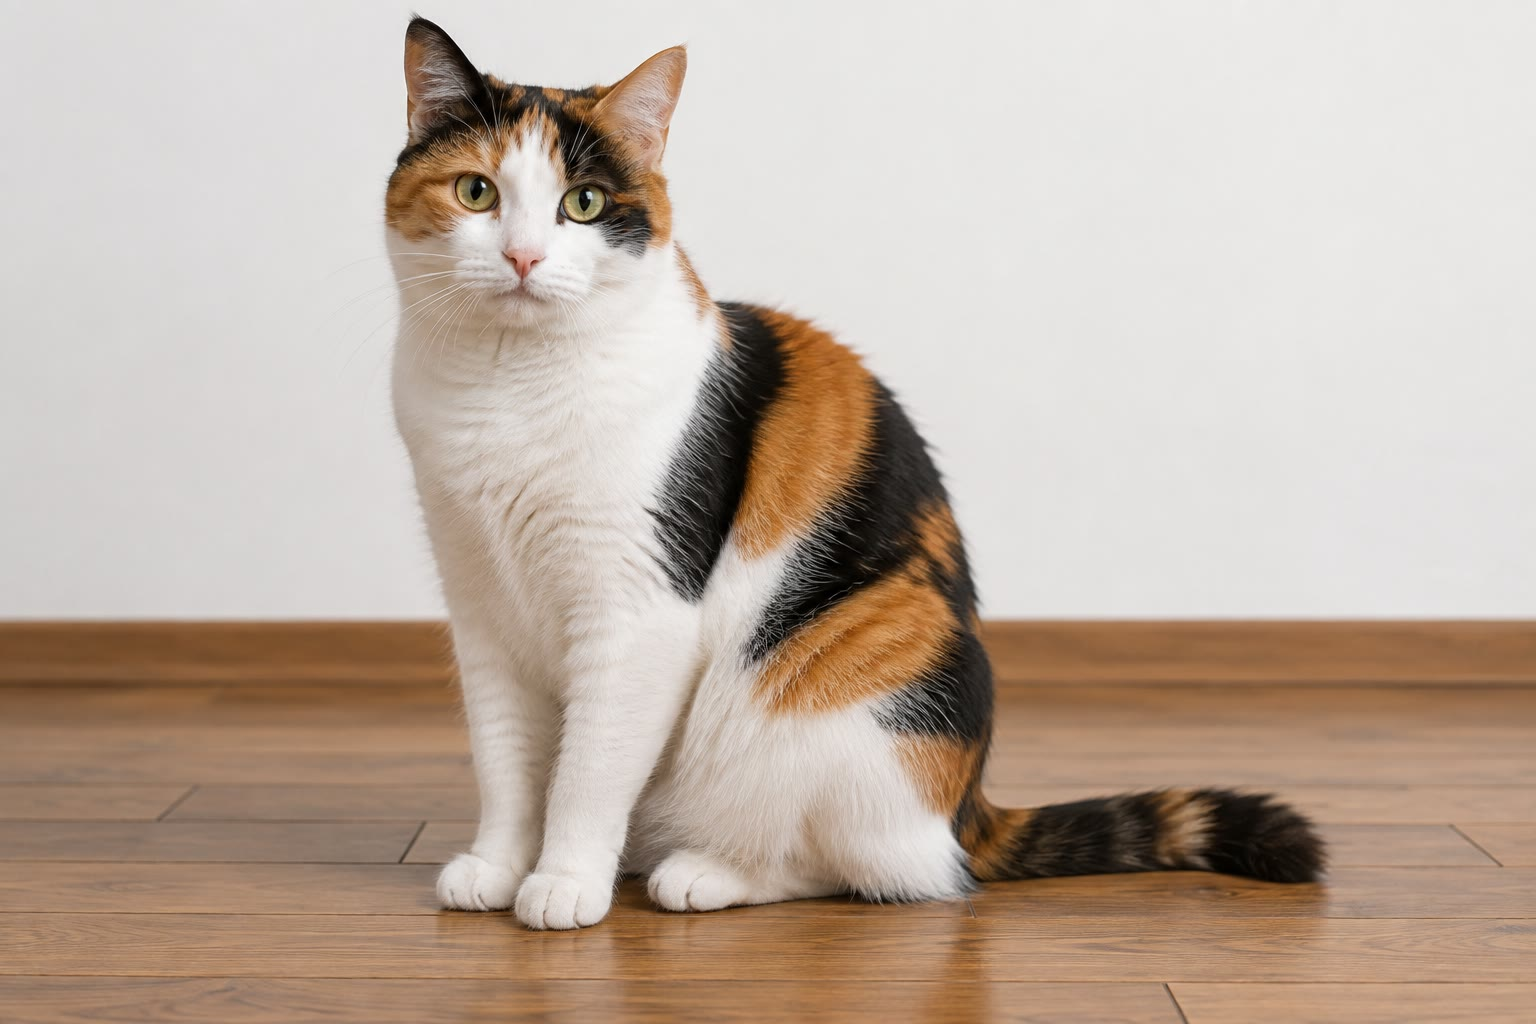
\includegraphics[width=0.5\linewidth]{images/book5/ai/b5-01-calico-cat.jpg}

{\small À gauche~: un noyau de femelle coloré pour l'ADN, avec l'X
inactif compact --- le \omterm{def:b3:chromatin-epigenetics:x-inactivation}{corpuscule de Barr} --- plaqué contre le bord du
noyau. À droite~: une chatte tricolore. Chaque plage orange ou noire
est un clone de cellules cutanées ayant réprimé le même chromosome~X~;
le blanc relève d'un autre gène, autosomique, de panachure.}
\end{omfigure}

\begin{definition}[Empreinte parentale]\label{def:b3:chromatin-epigenetics:imprinting}
\index{empreinte parentale}\index{région de contrôle de l'empreinte}\index{disomie uniparentale}
Un gène est soumis à l'\emph{empreinte} lorsqu'un seul de ses deux
allèles est exprimé, et que lequel dépend du parent dont il vient~:
certains gènes ne s'expriment que depuis la copie paternelle, d'autres
que depuis la maternelle. Les mammifères comptent quelque
\numrange{100}{200} gènes soumis à l'empreinte, groupés en amas, chaque
amas gouverné par une \emph{région de contrôle de l'empreinte} (ICR)
méthylée sur l'un des allèles parentaux et non sur l'autre. La
méthylation est installée dans la lignée germinale --- un profil dans
le spermatozoïde, un autre dans l'ovocyte --- effacée dans les cellules
germinales de la génération suivante, puis réinstallée selon le sexe de
l'individu. Un enfant qui reçoit les deux copies d'un chromosome du
même parent (\emph{disomie uniparentale}) a donc une mauvaise dose des
gènes à empreinte qu'il porte, bien que sa séquence soit parfaitement
normale.
\end{definition}

\begin{proof}[Faits expérimentaux]
McGrath et Solter, et indépendamment Surani, Barton et Norris (1984),
ont fabriqué des zygotes de souris portant deux pronucléus maternels,
ou deux paternels, en transférant des pronucléus entre œufs fécondés.
Aucun des deux types ne s'est développé à terme, bien que chacun eût
deux jeux complets de chromosomes~: les embryons gynogénétiques
formaient un embryon convenable avec un placenta médiocre, les
androgénétiques un gros placenta et presque pas d'embryon. Les deux
génomes parentaux ne sont pas équivalents et tous deux sont
nécessaires. Cattanach et Kirk (1985) ont montré, à l'aide de \omterm{def:b3:chromatin-epigenetics:imprinting}{disomies
uniparentales} portant sur un chromosome donné, que cette
non-équivalence est cantonnée à des régions particulières de
chromosomes particuliers, là où les amas soumis à l'empreinte ont été
trouvés par la suite.
\end{proof}

\begin{example}[L'amas \emph{Igf2}--\emph{H19}]\label{ex:b3:chromatin-epigenetics:igf2}
\emph{Igf2}, un facteur de croissance fœtale, s'exprime depuis l'allèle
paternel~; son voisin \emph{H19}, un ARN non codant, depuis le
maternel. Entre eux se trouve l'ICR et, au-delà de \emph{H19}, un jeu
d'amplificateurs communs. Sur le chromosome maternel l'ICR n'est pas
méthylée et fixe CTCF, qui agit en isolateur~: les amplificateurs
atteignent \emph{H19} mais pas \emph{Igf2}. Sur le chromosome paternel
l'ICR est méthylée (dans le spermatozoïde), CTCF ne peut s'y fixer, et
les amplificateurs atteignent \emph{Igf2}~; la méthylation se propage
en outre jusqu'à réprimer le promoteur de \emph{H19}. Une seule marque,
installée dans une seule lignée germinale, décide des deux gènes.
\end{example}

\begin{omfigure}
\begin{tikzpicture}[every node/.style={font=\scriptsize}, >=stealth]
  \foreach \yy/\lab/\ctcf in {1.6/chromosome maternel/1, -0.6/chromosome paternel/0} {
    \draw[very thick, gray] (0,\yy) -- (9.4,\yy);
    \node[left, align=right] at (-0.15,\yy) {\lab};
    \draw[thick, fill=omDef!25] (1.0,\yy-0.2) rectangle (2.6,\yy+0.2); \node at (1.8,\yy) {\emph{Igf2}};
    \draw[thick, fill=omProp!30] (4.2,\yy-0.2) rectangle (5.2,\yy+0.2); \node at (4.7,\yy) {ICR};
    \draw[thick, fill=omDef!25] (6.2,\yy-0.2) rectangle (7.4,\yy+0.2); \node at (6.8,\yy) {\emph{H19}};
    \foreach \x in {8.4,8.8,9.2} \fill[omMeth!70!black] (\x,\yy) circle (0.12);
    \node[right] at (9.55,\yy) {amplificateurs};
  }
  % maternal: CTCF bound, enhancer -> H19
  \draw[thick, fill=omExo!35] (4.7,2.15) ellipse (0.45 and 0.22); \node at (4.7,2.15) {CTCF};
  \draw[->, thick, omMeth!70!black] (8.4,1.85) .. controls (7.8,2.5) and (7.2,2.5) .. (6.8,1.85);
  \node[above] at (7.6,2.35) {actif};
  \draw[thick, omThm] (5.3,2.3) -- (5.3,0.9); \node[omThm, below] at (5.3,0.9) {isolateur};
  \node[omThm, above=1.0cm, align=center, font=\scriptsize] at (1.8,1.8) {\emph{Igf2} silencieux};
  % paternal: ICR methylated
  \foreach \x in {4.35,4.6,4.85,5.1} \fill[omThm] (\x,-0.95) circle (0.08);
  \node[below, align=center] at (4.7,-1.05) {méthylée~:\\pas de CTCF};
  \draw[->, thick, omMeth!70!black] (8.4,-0.35) .. controls (6.5,0.6) and (3.5,0.6) .. (1.8,-0.35);
  \node[above] at (3.3,0.2) {actif};
  \foreach \x in {6.4,6.7,7.0,7.2} \fill[omThm] (\x,-0.95) circle (0.08);
  \node[below] at (6.8,-1.05) {réprimé};
\end{tikzpicture}

{\small L'empreinte en \emph{Igf2}--\emph{H19}. Allèle maternel~: l'ICR
non méthylée fixe CTCF, un isolateur, de sorte que les amplificateurs
situés en aval n'activent que \emph{H19}. Allèle paternel~: l'ICR a été
méthylée dans le spermatozoïde, CTCF ne peut s'y fixer, les
amplificateurs atteignent \emph{Igf2}, et la méthylation réprime
\emph{H19}.}
\end{omfigure}

\begin{example}[Prader--Willi et Angelman]\label{ex:b3:chromatin-epigenetics:pws}
La même délétion d'environ \qty{5}{Mb} du chromosome~15 (région
15q11--q13) cause le \emph{syndrome de Prader--Willi} --- hypotonie
musculaire à la naissance, puis appétit insatiable et obésité ---
lorsqu'elle est portée par le chromosome paternel, et le \emph{syndrome
d'Angelman} --- déficience intellectuelle sévère, absence de langage,
humeur joyeuse et crises convulsives --- lorsqu'elle est portée par le
maternel. La région contient des gènes à expression paternelle
(\emph{SNRPN} et un amas de petits ARN) dont la seule copie active est
perdue dans le premier cas, et le gène à expression maternelle
\emph{UBE3A}, perdu dans le second. Une \omterm{def:b3:chromatin-epigenetics:imprinting}{disomie uniparentale} maternelle
du~15, sans aucune délétion, donne également un Prader--Willi~: deux
copies maternelles, silencieuses pour les gènes paternels.
\end{example}

\begin{remark}[Pourquoi une empreinte]\label{rem:b3:chromatin-epigenetics:kinship}
Les gènes soumis à l'empreinte sont enrichis en fonctions de contrôle
de la croissance fœtale et du transfert de nutriments par le placenta,
ceux à expression paternelle (\emph{Igf2}, \emph{Peg3}) tendant à
favoriser la croissance et ceux à expression maternelle (\emph{H19},
\emph{Igf2r}, \emph{Cdkn1c}) à la freiner. La \emph{théorie du conflit
de parentèle} y lit un conflit~: les gènes d'un père gagnent à extraire
davantage d'une mère qui portera peut-être plus tard les petits
d'autres mâles, tandis que les gènes de la mère gagnent à rationner
entre toutes ses portées. L'empreinte existe chez les mammifères
placentaires et chez les plantes à fleurs, dont l'albumen est lui aussi
nourri par la mère, et non chez les oiseaux ni chez les reptiles, ce
qui est bien ce que la théorie prédit.
\end{remark}

\section{Hérédité épigénétique et ses limites}

\begin{definition}[Épigénétique]\label{def:b3:chromatin-epigenetics:epigenetics}
\index{épigénétique}\index{épiallèle}\index{reprogrammation}
L'\emph{épigénétique} est l'étude des changements héritables de
l'activité des gènes qui ne sont pas des changements de la séquence de
l'ADN~: des états portés par la \omterm{def:b3:chromatin-epigenetics:methylation}{méthylation de l'ADN}, par les marques
d'\omterm{def:b3:chromatin-epigenetics:nucleosome}{histones} ou par des circuits de facteurs de transcription
auto-entretenus, et recopiés au travers de la division cellulaire. Deux
allèles de séquence identique mais d'état épigénétique stable
différent sont des \emph{épiallèles}. L'hérédité au travers de la
mitose est la règle, et c'est elle qui fait qu'une cellule
différenciée le reste. L'hérédité au travers de la méiose, du parent à
sa descendance, est l'exception chez les mammifères, car les marques
sont effacées en deux vagues de \emph{reprogrammation}~: dans les
cellules germinales primordiales, où les empreintes et la plus grande
partie de la méthylation sont gommées puis réinstallées selon le sexe,
et de nouveau dans le zygote et l'embryon précoce, où le génome
paternel est déméthylé activement par TET3 et le maternel passivement,
avant que les profils propres à l'embryon ne soient posés par DNMT3.
\end{definition}

\begin{example}[La souris agouti viable jaune]\label{ex:b3:chromatin-epigenetics:agouti}
Dans l'allèle $A^{vy}$, un rétrotransposon s'est inséré en amont du
gène de couleur du pelage \emph{agouti}. Là où le promoteur du
transposon n'est pas méthylé, il exprime \emph{agouti} en permanence
dans toutes les cellules~; la souris est jaune, obèse et sujette au
diabète. Là où il est méthylé, le gène suit son contrôle normal et la
souris est brune («~pseudoagouti~»). Des sœurs de portée génétiquement
identiques couvrent tout le spectre, et une mère jaune a plus de petits
jaunes qu'une mère brune~: l'\omterm{def:b3:chromatin-epigenetics:epigenetics}{épiallèle} n'est qu'incomplètement effacé
au travers de la lignée germinale maternelle. Waterland et Jirtle
(2003) ont nourri des mères $A^{vy}$ gestantes avec un régime riche en
donneurs de méthyle (folates, vitamine B\textsubscript{12}, choline,
bétaïne) et ont déplacé le pelage des petits vers le brun.
L'environnement d'une génération avait installé une marque que la
suivante a portée.
\end{example}

\begin{omfigure}
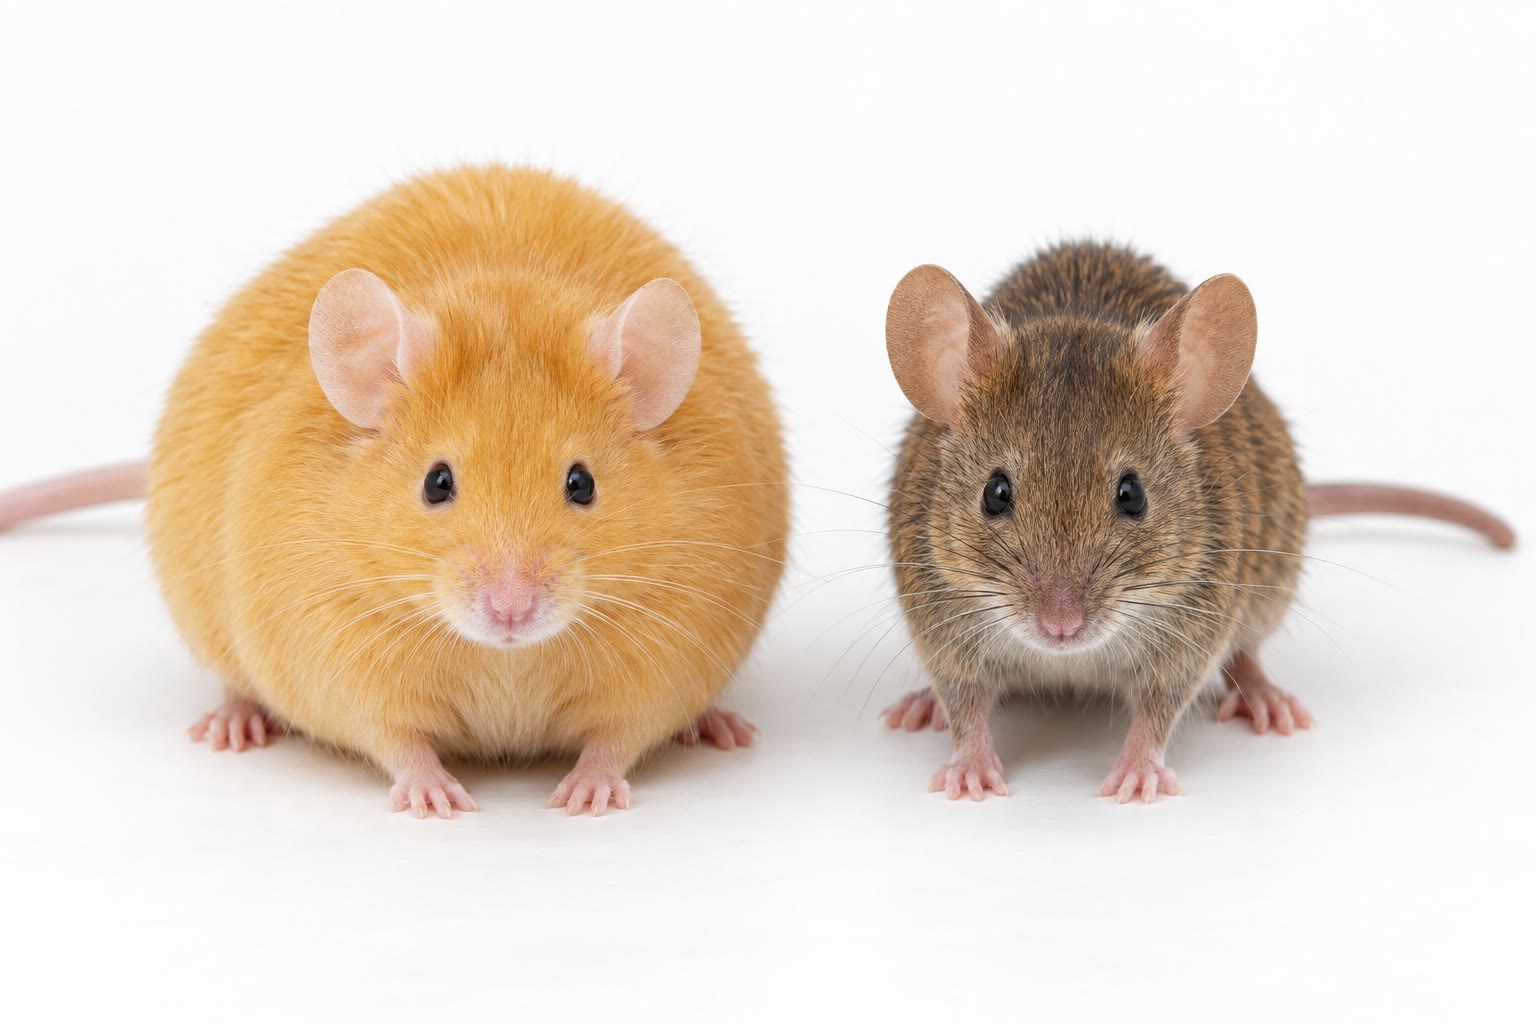
\includegraphics[width=0.62\linewidth]{images/book5/ai/b5-01-agouti-mice.jpg}

{\small Deux sœurs de portée $A^{vy}$ de génotype identique~: une
souris jaune et obèse, chez qui le transposon situé en amont
d'\emph{agouti} n'est pas méthylé, et une pseudoagouti brune, chez qui
il l'est.}
\end{omfigure}

\begin{proposition}[Où l'on trouve des états épigénétiques héritables]\label{prop:b3:chromatin-epigenetics:examples}
\index{panachure par effet de position}\index{vernalisation}\index{paramutation}
Trois systèmes bien analysés illustrent les mécanismes ci-dessus. La
\emph{\omterm{prop:b3:chromatin-epigenetics:examples}{panachure par effet de position}} chez la \emph{drosophile}~: un
gène déplacé par un remaniement chromosomique au voisinage de
l'\omterm{def:b3:chromatin-epigenetics:nucleosome}{hétérochromatine} est réprimé dans certaines cellules et non dans
d'autres, ce qui donne un œil marbré~; chaque plage est un clone, la
répression se propage depuis l'\omterm{def:b3:chromatin-epigenetics:nucleosome}{hétérochromatine} par la boucle HP1, et
les gènes dont la mutation supprime la panachure (gènes
\emph{Su(var)}) sont HP1 et la méthyltransférase de H3K9. La
\emph{vernalisation} chez \emph{Arabidopsis}~: des semaines de froid
hivernal répriment le répresseur de floraison \emph{FLC} par la marque
H3K27me3 déposée par Polycomb, le silence tient au long des mois de
croissance printanière et de milliers de divisions cellulaires, et il
est remis à zéro à chaque génération, si bien que chaque plante doit
connaître son propre hiver. La \emph{paramutation} chez le maïs~: un
allèle du gène de pigmentation \emph{b1}, lorsqu'il rencontre un autre
allèle particulier chez un hétérozygote, le convertit à son propre état
silencieux, et l'allèle converti transmet cet état à sa descendance
pendant des générations, par une méthylation dirigée par de petits ARN
reprise au \cref{ch:b3:rna-regulation}. Dans chaque cas l'hérédité
mitotique est robuste~; la transmission entre générations est soit
activement remise à zéro (plantes), soit partielle et fuyante (souris).
\end{proposition}

\begin{remark}[Les limites des affirmations transgénérationnelles]\label{rem:b3:chromatin-epigenetics:limits}
L'affirmation que la famine ou le stress d'un grand-parent serait
«~hérité épigénétiquement~» par des petits-enfants humains est
courante et le plus souvent non démontrée. Deux vagues d'effacement
séparent une marque somatique d'un petit-enfant, les gènes soumis à
l'empreinte et quelques transposons sont les seuls survivants
documentés de l'effacement chez les mammifères, et dans les cohortes
humaines les effets d'un environnement partagé, de l'environnement
utérin et des différences génétiques sont difficiles à séparer d'une
marque portée par la lignée germinale. Les cas démontrés --- $A^{vy}$,
quelques \omterm{def:b3:chromatin-epigenetics:epigenetics}{épiallèles} liés à un transposon, des états portés par des ARN
chez les vers et les plantes --- sont réels, compris au niveau
moléculaire, et peu nombreux. Le théorème du chapitre dit pourquoi~:
sans rétroaction poussant $\mu$ vers $1$, une marque s'oublie en
quelques dizaines de divisions, et la lignée germinale y ajoute une
remise à zéro active.
\end{remark}

\section{Exercices}

\begin{exercise}[$\star$]\label{exo:b3:chromatin-epigenetics:1}
Donner la composition d'une particule cœur de \omterm{def:b3:chromatin-epigenetics:nucleosome}{nucléosome}, la longueur
d'ADN qu'elle fixe et la longueur habituelle de l'ADN de liaison.
Pourquoi la digestion de la \omterm{def:b3:chromatin-epigenetics:nucleosome}{chromatine} par une nucléase donne-t-elle
une échelle de fragments plutôt qu'une traînée continue~?
\end{exercise}

\begin{exercise}[$\star$]\label{exo:b3:chromatin-epigenetics:2}
Un génome de grenouille compte $3.0\times 10^{9}$ paires de bases par
jeu haploïde. Combien de \omterm{def:b3:chromatin-epigenetics:nucleosome}{nucléosomes} un noyau diploïde contient-il,
pour une répétition de \qty{190}{bp}, et quelle est la longueur de son
ADN~?
\end{exercise}

\begin{exercise}[$\star$]\label{exo:b3:chromatin-epigenetics:3}
Décoder H3K27me3, H4K16ac et H3S10ph. Dire pour chacune si elle est
associée à une \omterm{def:b3:chromatin-epigenetics:nucleosome}{chromatine} active ou silencieuse, et nommer un \omterm{def:b3:chromatin-epigenetics:histone-code}{lecteur}
de la première.
\end{exercise}

\begin{exercise}[$\star$]\label{exo:b3:chromatin-epigenetics:4}
Expliquer pourquoi un chat tricolore est presque toujours une femelle,
et ce que doit être un mâle tricolore.
\end{exercise}

\begin{exercise}[$\star\star$]\label{exo:b3:chromatin-epigenetics:5}
Calculer le \omterm{prop:b3:chromatin-epigenetics:compaction}{taux de compaction} de la fibre de \qty{10}{nm} à partir des
nombres de la \cref{def:b3:chromatin-epigenetics:nucleosome}
(répétition \qty{200}{bp}, perle \qty{11}{nm}), puis le taux nécessaire
pour loger les \qty{4}{cm} d'ADN d'un chromosome humain moyen dans une
chromatide mitotique longue de \qty{4}{\micro m}. De quel facteur
supplémentaire la fibre doit-elle être repliée~?
\end{exercise}

\begin{exercise}[$\star\star$]\label{exo:b3:chromatin-epigenetics:6}
Dans le modèle du \cref{thm:b3:chromatin-epigenetics:maintenance} avec
$\mu = 0.98$ et $\delta = 0.01$, trouver $p^{*}$ et le nombre de
divisions au bout duquel un site parti méthylé a perdu la moitié de son
excès sur $p^{*}$. Recommencer pour $\mu = 0.999$, $\delta = 0.001$.
\end{exercise}

\begin{exercise}[$\star\star$]\label{exo:b3:chromatin-epigenetics:7}
Une expérience de ChIP-seq sur des cellules de foie donne un pic
H3K4me3 et un pic H3K27ac au promoteur du gène $A$, un large domaine
H3K27me3 sur le gène $B$, et H3K9me3 sur le gène $C$. Prévoir l'état
transcriptionnel de chacun, et dire lequel de $B$ et de $C$ a le plus
de chances d'être activé dans un autre type cellulaire, et pourquoi.
\end{exercise}

\begin{exercise}[$\star\star$]\label{exo:b3:chromatin-epigenetics:8}
Une femme porte une délétion de la région \emph{UBE3A} sur l'un de ses
chromosomes~15 mais se porte bien. Son père portait la même délétion et
se portait bien lui aussi. De quel syndrome, s'il y en a un, chacun de
ses enfants risque-t-il d'être atteint, et avec quelle probabilité~? Et
si la délétion lui était venue de sa mère~?
\end{exercise}

\begin{exercise}[$\star\star$]\label{exo:b3:chromatin-epigenetics:9}
Prévoir la conséquence, chez un embryon de souris femelle, de la
délétion du gène \emph{\omterm{def:b3:chromatin-epigenetics:x-inactivation}{Xist}} sur un chromosome~X, puis sur les deux.
Prévoir ce qu'un transgène \emph{\omterm{def:b3:chromatin-epigenetics:x-inactivation}{Xist}} inséré dans un autosome fait à
cet autosome.
\end{exercise}

\begin{exercise}[$\star\star\star$]\label{exo:b3:chromatin-epigenetics:10}
Expliquer, à l'aide de l'\cref{ex:b3:chromatin-epigenetics:cpg-deficit},
pourquoi les \omterm{def:b3:chromatin-epigenetics:methylation}{îlots CpG} ont gardé leurs \omterm{def:b3:chromatin-epigenetics:methylation}{CpG} alors que le reste du génome
en a perdu les quatre cinquièmes, et ce que cela implique quant à
l'état de méthylation des îlots dans la lignée germinale au fil du
temps évolutif. Pourquoi l'argument tombe-t-il pour un gène méthylé
seulement dans le foie~?
\end{exercise}

\begin{exercise}[$\star\star\star$]\label{exo:b3:chromatin-epigenetics:11}
Montrer, à l'aide de la boucle écrivain--lecteur de la
\cref{prop:b3:chromatin-epigenetics:readers}, comment un domaine
H3K9me3 peut être stable au travers de la réplication, alors que chaque
division dilue de moitié les \omterm{def:b3:chromatin-epigenetics:nucleosome}{histones} marquées avec des \omterm{def:b3:chromatin-epigenetics:nucleosome}{histones} neuves
non marquées. Qu'est-ce qui détermine où la propagation du domaine
s'arrête~? Proposer une expérience pour tester cette explication.
\end{exercise}

\begin{exercise}[$\star\star\star$]\label{exo:b3:chromatin-epigenetics:12}
Une étude rapporte que les petits-enfants de personnes ayant vécu une
famine présentent une méthylation modifiée sur un gène de croissance et
une masse corporelle plus élevée. Énumérer les explications de rechange
qu'il faut écarter avant de conclure qu'une marque de méthylation a été
transmise par la lignée germinale, et dire quelle expérience chez la
souris trancherait la question.
\end{exercise}

\section{Problème~: la mémoire d'un gène réprimé}

\begin{problem}[{Problème du week-end --- un génome humain rangé dans
son noyau, une marque de méthylation suivie au fil des divisions, une
chatte tricolore lue comme une carte clonale et les maladies d'une
région soumise à l'empreinte dénombrées, pour finir sur le nombre de
divisions qu'une marque survit sans rétroaction et sur la taille de la
population cellulaire qui a choisi son X}]
\label{pb:b3:chromatin-epigenetics:1}
Données~: un noyau diploïde humain contient $6.4\times 10^{9}$ paires
de bases, à \qty{0.34}{nm} et \qty{650}{Da} la paire~; la répétition
nucléosomique est de \qty{200}{bp}, un octamère d'\omterm{def:b3:chromatin-epigenetics:nucleosome}{histones} pèse
\qty{108}{kDa}, et une particule cœur est un disque de \qty{11}{nm} de
diamètre et \qty{5.5}{nm} d'épaisseur. Le noyau est une sphère de
\qty{10}{\micro m} de diamètre. Le génome contient \qty{42}{\%} de
G$+$C. Méthylation d'un \omterm{def:b3:chromatin-epigenetics:methylation}{CpG} ordinaire~: $\mu = 0.99$, $\delta = 0.02$
par division.

\medskip
\noindent\textbf{Partie I --- L'emballage.}
\begin{enumerate}
  \item Calculer la longueur totale d'ADN du noyau et le nombre de
        \omterm{def:b3:chromatin-epigenetics:nucleosome}{nucléosomes}.
  \item Calculer la masse totale d'\omterm{def:b3:chromatin-epigenetics:nucleosome}{histones} (octamères seuls) et celle
        d'ADN, en picogrammes ($\qty{1}{Da} = \qty{1.66e-24}{g}$).
  \item Calculer le volume du noyau et le volume total des particules
        cœur, traitées comme des cylindres. Quelle fraction du noyau
        occupent-elles~?
  \item Si les \omterm{def:b3:chromatin-epigenetics:nucleosome}{nucléosomes} étaient mis bout à bout en une fibre de
        \qty{10}{nm}, quelle serait la longueur de la fibre, et quel
        est le \omterm{prop:b3:chromatin-epigenetics:compaction}{taux de compaction} par rapport à l'ADN nu~?
  \item La fibre est repliée en boucles de \qty{200}{kb} ancrées par la
        cohésine. Combien de boucles, et combien de \omterm{def:b3:chromatin-epigenetics:nucleosome}{nucléosomes} par
        boucle~?
  \item Sous l'hypothèse d'indépendance, combien de dinucléotides \omterm{def:b3:chromatin-epigenetics:methylation}{CpG}
        le génome diploïde contiendrait-il~? Le nombre observé est
        $5.6\times 10^{7}$. Quelle fraction a été perdue, et par quel
        mécanisme mutationnel~?
\end{enumerate}

\medskip
\noindent\textbf{Partie II --- Une marque au fil des divisions.}
\begin{enumerate}[resume]
  \item Écrire la récurrence pour $p_{n}$ et calculer $p^{*}$.
  \item Un \omterm{def:b3:chromatin-epigenetics:methylation}{CpG} de promoteur est entièrement méthylé en $n = 0$.
        Calculer $p_{n}$ après $10$, $50$ et $200$ divisions.
  \item Au bout de combien de divisions l'excès $p_{n} - p^{*}$ est-il
        divisé par deux~? Une cellule souche de tissu se divise environ
        une fois par semaine~: cela fait combien d'années~?
  \item Un médicament inhibe complètement \omterm{def:b3:chromatin-epigenetics:methylation}{DNMT1} ($\mu = 0$) ainsi que
        DNMT3 ($\delta = 0$). Montrer que la fraction de brins méthylés
        dans la population est divisée par deux à chaque division, et
        trouver le nombre de divisions qui fait passer une méthylation
        de \qty{80}{\%} sous \qty{5}{\%}.
  \item Dans un îlot réprimé, les \omterm{def:b3:chromatin-epigenetics:histone-code}{lecteurs} du \omterm{def:b3:chromatin-epigenetics:methylation}{méthyl-CpG} recrutent la
        méthylation de H3K9, qui recrute DNMT3, si bien qu'au sein de
        l'îlot $\mu = 0.9995$ et $\delta = 0.0005$. Recalculer la
        demi-vie de l'excès, en divisions et en années à une division
        par semaine.
  \item Expliquer en une phrase pourquoi c'est le résultat de la
        question 11, et non celui de la question 9, qu'exige un gène
        réprimé à vie, et quel genre d'arrangement moléculaire le
        produit.
\end{enumerate}

\medskip
\noindent\textbf{Partie III --- La carte tricolore.}
\begin{enumerate}[resume]
  \item Une chatte est hétérozygote pour le gène orange lié à l'X.
        Expliquer pourquoi son pelage porte des plages orange et
        noires, et ce que représente une plage.
  \item L'\omterm{def:b3:chromatin-epigenetics:x-inactivation}{inactivation de l'X} a eu lieu quand les cellules destinées à
        former la peau étaient au nombre de $N$. Chacune a choisi un X
        au hasard. Quelle est la probabilité qu'elles aient toutes les
        $N$ choisi le même, donnant une chatte d'une seule couleur~?
  \item Aucune hétérozygote d'une seule couleur n'a été documentée
        parmi peut-être un milliard de chats~; prendre la probabilité
        égale à $10^{-9}$ et estimer $N$.
  \item La surface cutanée de la chatte vaut environ \qty{0.3}{m^2} et
        ses plages \qty{15}{cm^2} en moyenne. Estimer le nombre de
        plages et expliquer pourquoi il est supérieur à $N$.
  \item Un chat XXY est lui aussi tricolore. Combien de \omterm{def:b3:chromatin-epigenetics:x-inactivation}{corpuscules de
        Barr} ses cellules montrent-elles~? Et combien chez une femelle
        XXX et chez un mâle XY~?
  \item Un gène qui échappe à l'inactivation est présent en deux copies
        actives chez les femelles et en une seule chez les mâles.
        Donner une raison pour laquelle un tel échappement peut être
        toléré, et une situation où il compte.
\end{enumerate}

\medskip
\noindent\textbf{Partie IV --- Le chromosome~15.}
\begin{enumerate}[resume]
  \item Le syndrome de Prader--Willi touche environ une naissance sur
        \num{15000}~; \qty{70}{\%} des cas sont une délétion de novo du
        15q11--q13 paternel et \qty{25}{\%} une \omterm{def:b3:chromatin-epigenetics:imprinting}{disomie uniparentale}
        maternelle. Calculer la fréquence à la naissance de chaque
        cause.
  \item Le syndrome d'Angelman a à peu près la même fréquence~;
        \qty{70}{\%} sont des délétions maternelles, \qty{5}{\%} des
        disomies paternelles et \qty{10}{\%} des mutations ponctuelles
        d'\emph{UBE3A}. Pourquoi les mutations ponctuelles causent-elles
        un Angelman mais presque jamais un Prader--Willi~?
  \item Un père porte une translocation équilibrée qui donne à
        \qty{20}{\%} de ses spermatozoïdes une délétion 15q11--q13.
        Quelle fraction de ses enfants a un Prader--Willi, et quelle
        fraction un Angelman~?
  \item Une \omterm{def:b3:chromatin-epigenetics:imprinting}{disomie uniparentale} apparaît lorsqu'un zygote trisomique
        perd un chromosome. Si un zygote trisomique~15 perd au hasard
        l'un de ses trois chromosomes, et que la trisomie vient de la
        mère (deux copies maternelles), quelle est la probabilité que
        le survivant porte une disomie maternelle~? Quel syndrome~?
  \item Les gènes de Prader--Willi sont à expression paternelle et
        celui d'Angelman à expression maternelle. À l'aide de la
        théorie du conflit de parentèle, dire lesquels des symptômes
        des deux syndromes (difficulté à téter à la naissance contre
        appétit vorace) cadrent avec la théorie et lesquels sont plus
        difficiles à y faire entrer.
  \item On propose une méthode pour traiter l'Angelman en réactivant
        l'\emph{UBE3A} paternel silencieux. Son silence est dû à un ARN
        antisens à expression paternelle. Proposer la cible moléculaire
        et dire pourquoi la thérapie ne perturberait pas les autres
        gènes soumis à l'empreinte.
  \item Résumer~: la demi-vie d'une marque sans rétroaction
        (question~9) et avec elle (question~11), en divisions~; et la
        population fondatrice $N$ du pelage tricolore (question~15).
\end{enumerate}
\end{problem}
